\scanpage{10}
sous $u$ sont celles contenues dans un de ces sous-espaces. Si on veut qu'elles soient aussi inv. sous $\sigma$, il ne reste plus que les droites \unsure{des|dans} les deux premiers sous-espaces. Or on est en car. $\ne2$ (car ${\unsure{\zeta|\xi}}^2=-1$, mais $\zeta^2\ne+1$ fibre par fibre) et $\sigma$ opère sur $\check D_1^{\otimes2}\oplus\check D_2^{\otimes2}$ en permutant $\check D_1^{\otimes2}$ et $\check D_2^{\otimes2}\ldots$ Cela fait donc $2$ droites propres exactement de l'espace qu'ils engendrent, correspondant aux val. propres $+1$ et $-1$ resp. pour $\sigma$, les val. propres pour $u$ étant $-1,-1$, celles pour $\sigma'\inserted{=u\sigma}$ \deleted{étant} donc $-1,1$.

Si on \deleted{\unsure{expr|appr}} récrit le cadre en coordonnées $(x,y)$ avec sommets $(\pm1,\pm1)$ \deleted{\unsure{du carré|de côtés}} se suivant dans l'ordre
\[
(1,1),(-1,1),(-1,-1),(1,-1)
\]
\figure{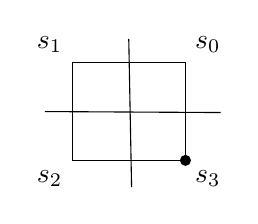
\begin{tikzpicture}[x=.72cm,y=.62cm]
\draw (-1,1)--(1,1)--(1,-1)--(-1,-1)--cycle;
\draw (-1.48,0)--(1.62,-.02); \draw (0,1.49)--(.05,-1.55);
\fill (1,-1) circle (2pt);
\node[above left] at (-1,1) {$s_1$}; \node[above right] at (1,1) {$s_0$};
\node[below left] at (-1,-1) {$s_2$}; \node[below right] at (1,-1) {$s_3$};
\end{tikzpicture}}
\margin{\uline{NB} car $\ne2$}
Les formes quadratiques en $(x,y,z)$ correspondantes sont $x^2-y^2\inserted{=(x-y)(x+y)}$ et $xy$ (\uline{NB} $\sigma(x,y)=(y,x)$ $\sigma'(x,y)=(-x,y)$).

\deleted{\uline{elles sont toutes deux \inserted{non} dégénérées}.} [La première prend la valeur constante \deleted{\unsure{$4$|$\ne$}}$0$ sur les sommets du carré, la seconde prend la valeur $+1$ sur \inserted{un couple de} deux sommets opposés, la valeur $-1$ sur le couple des deux autres sommets... ] Seule la première définit une conique inv. passant par les sommets du carré, savoir la
% archive sheet number: 9
